\chapter{代码阅读} 
\label{ch:code-reading}

\begin{content}

在程序员的日常工作之中,绝大多数时间都是在\emph{阅读代码},而不是在写代码。但是,阅读代码往往是一件很枯燥的事情,尤其当遇到了一个不漂亮的设计,反抗的心理往往更加强烈。事实上,变换一下习惯、思路和方法,代码阅读其实是一个很享受的过程。

阅读代码的模式,实践和习惯,集大成者莫过于希腊作者\ascii{Diomidis Spinellis}的经典之作:\ascii{Code Reading, The Open Source Perspective}。本文从另外一个视角出发,谈谈我阅读代码的一些习惯,期待找到更多知音的共鸣。

\end{content}

\section{工欲善其事,必先利其器}

\begin{content}

首先,阅读代码之前先准备好一个称心如意的工具箱,包括\ascii{IDE}, \ascii{UML},脑图等工具。我主要使用的编程语言包括\ascii{C++, Scala, Java, Ruby, Python};我更偏向使用\ascii{JetBrains}公司的产品,其很多习惯用法对程序员都很贴心。

其次,高效地使用快捷键,这是一个良好的代码阅读习惯,它极大地提高了代码阅读的效率和质量。例如,查看类层次关系,函数调用链,方法引用点等等。

\begin{remark}
拔掉鼠标,减低对鼠标的依赖。当发现没有鼠标而导致工作无法进行下去时,尝试寻找对应的快捷键。通过日常的点滴积累,工作效率必然能够得到成倍的提高。
\end{remark}

\end{content}

\section{力行而后知之真}

\begin{content}

阅读代码一种常见的反模式就是通过\ascii{Debug}的方式来阅读代码。作者不推荐这种代码阅读的方式,其一,因为运行时线程间的切换很容易导致方向的迷失;其二,了解代码调用栈对于理解系统行为并非见得有效,因为其包含太多实现细节,不易发现问题的本质。

但在阅读代码之前,有几件事情是必须做的。其一,手动地构建一次工程,并运行测试用例;其二,亲自动手写几个\ascii{Demo}感受一下。

先将工程跑起来,目的不是为了\ascii{Debug}代码,而是在于了解工程构建的方式,及其认识系统的基本结构,并体会系统的使用方式。

如果条件允许,可以尝试使用\ascii{ATDD}的方式,发现和挖掘系统的行为。通过这个过程,将自己当成一个客户,思考系统的行为,这是理解系统最重要的基石。

\end{content}

\section{发现领域模型}

\begin{content}

阅读代码,不是为了了解每个类,每个函数干什么,而是为了挖掘更本质,更不易变化的知识。事实上,发现\emph{领域模型}是阅读代码最重要的一个目标,因为领域模型是系统的灵魂所在。通过代码阅读,找到系统本质的知识,并通过自己的模式表达出来,才能真正地抓住系统的脉络,否则一切都是空谈。

例如,在阅读\tf{}的\ascii{Python}实现的客户端代码时,理顺计算图的领域模型,对于理解\ascii{TensorFlow}的编程模型,及其系统运行时的行为极其重要。

\begin{figure}[!htbp]
\centering
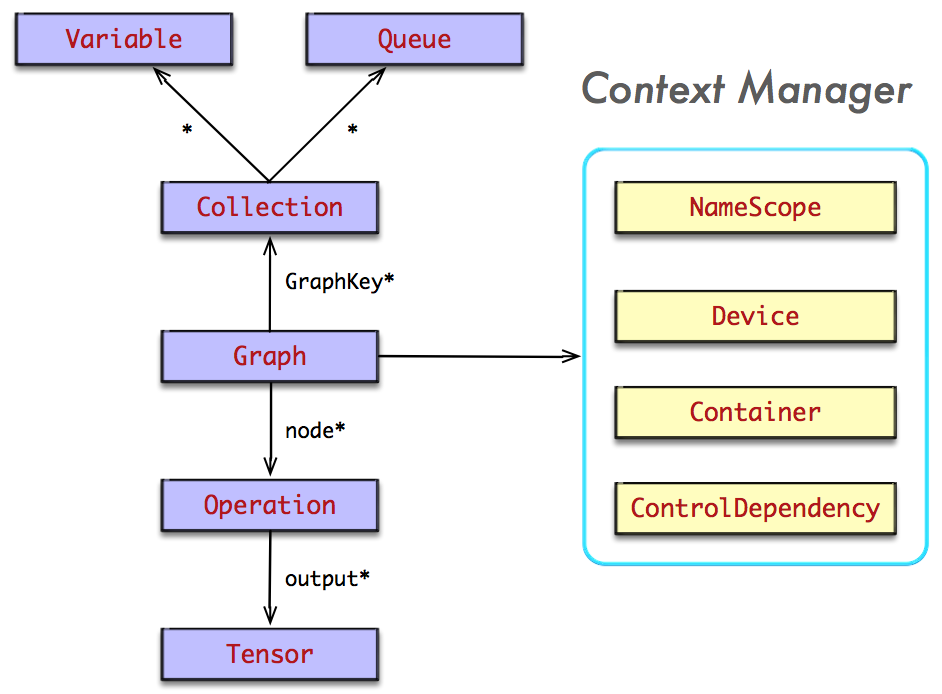
\includegraphics[width=0.9\textwidth]{figures/py-graph.png}
\caption{领域对象:Graph}
 \label{fig:py-graph}
\end{figure}

\end{content}

\section{挖掘系统架构}

\begin{content}

阅读代码犹如在大海中航行,系统架构图就是航海图。阅读代码不能没有整体的系统概念,否则收效不佳,阅读质量大大折扣。必须拥有系统思维,并明确目标,才不至于迷失方向。

首要的任务,就是找到系统的边界,并能够以抽象的思维思考外部系统的行为特征。其次,理清系统中各组件之间的交互,关联关系,及其职责,对于理解整个系统的行为极为重要。

例如,对于\ascii{TensorFlow},\ascii{C API}是衔接前后端系统的桥梁。理解\ascii{C API}的设计,基本能够猜测前后端系统的行为。

\begin{figure}[!h]
\centering
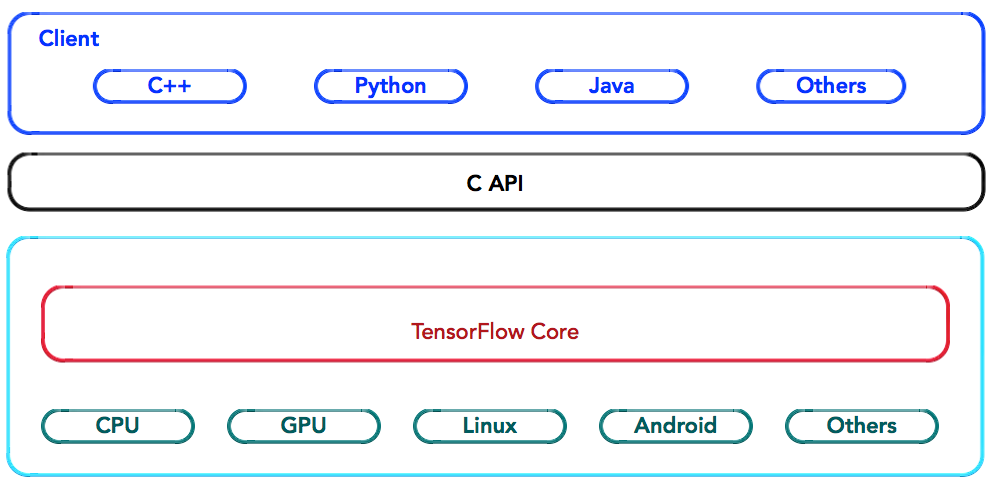
\includegraphics[width=0.9\textwidth]{figures/tf-architecture-simple.png}
\caption{TensorFlow系统架构}
 \label{fig:tf-architecture-simple}
\end{figure}

\end{content}

\section{细节是魔鬼}

\begin{content}

纠结于细节,将导致代码阅读代码的效率和质量大大折扣。例如,日志打印,解决某个\ascii{Bug}的补丁实现,某版本分支的兼容方案,某些变态需求的锤子代码实现等等。

阅读代码的一个常见的反模式就是「给代码做批注」。这是一个高耗低效,投入产出比极低的实践。一般地,越是优雅的系统,注释越少;越是复杂的系统,再多的注释也是于事无补。

我有一个代码阅读的习惯,为代码阅读建立一个单独的\ascii{code-reading}分支,一边阅读代码,一边删除这些无关的代码。

\begin{leftbar}
\begin{scala}
$ git checkout -b code-reading
\end{scala}
\end{leftbar}

删除这些噪声后,你会发现系统根本没有想象之中那么复杂。现实中,系统的复杂性,往往都是不成熟的设计和实现导致的额外复杂度。随着对系统的深入理解,很多细节都会自然地浮出水面,所有神秘的面纱都将被揭开而公示天下。

\end{content}

\section{适可而止}

\begin{content}

阅读代码的一个常见的反模式就是「一根筋走到底,不到黄河绝不死心」。程序员都拥有一颗好奇心,总是对不清楚的事情感兴趣。例如,消息是怎么发送出去的?任务调度工作原理是什么?数据存储怎么做到的?;虽然这种勇气值得赞扬,但在代码阅读时绝对不值得鼓励。

还有另外一个常见的反模式就是「追踪函数调用栈」。这是一个极度枯燥的过程,常常导致思维的僵化;因为你永远活在作者的阴影下,完全没有自我。

我个人阅读代码的时候,函数调用栈深度绝不超过\ascii{3},然后使用抽象的思维方式思考底层的调用。因为我发现,随着年龄的增长,曾今值得骄傲的记忆力,现在逐渐地变成自己的短板。当我尝试追踪过深的调用栈之后,之前的阅读信息完全地消失记忆了。

也就是说,我更习惯于「广度遍历」,而不习惯于「深度遍历」的阅读方式。这样,我才能找到系统隐晦存在的「分层概念」,并理顺系统的层次结构。

\end{content}

\section{发现她的美}

\begin{content}

三人行,必有我师焉。在代码阅读代码时,当发现好的设计,包括实现模式,习惯用法等,千万不要错过;否则过上一段时间,这次代码阅读对你来说就没有什么价值了。

当我发现一个好的设计时,我会尝试使用类图,状态机,序列图等方式来表达设计;如果发现潜在的不足,将自己的想法补充进去,将更加完美。

例如,当我阅读\ascii{Hamcrest}时,尝试画画类图,并体会它们之间关系,感受一下设计的美感,也是受益颇多的。

\begin{figure}[!h]
\centering
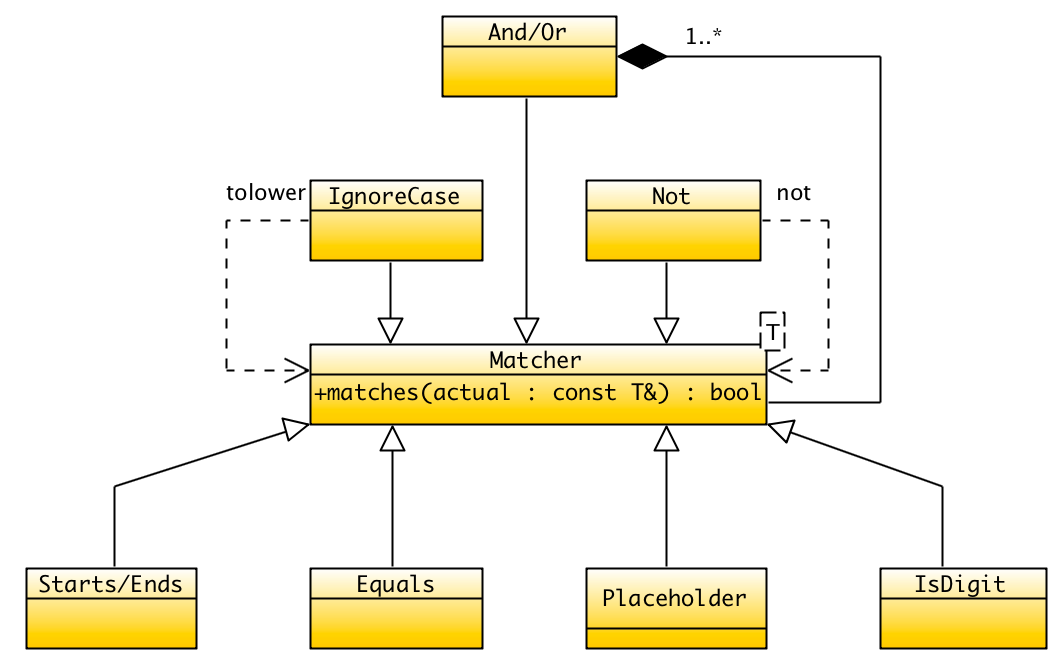
\includegraphics[width=0.9\textwidth]{figures/hamcrest.png}
\caption{组合式设计}
 \label{fig:hamcrest}
\end{figure}

\end{content}

\section{尝试重构}

\begin{content}

因为这是一次代码阅读的过程,不会因为重构带来潜在风险的问题。在一些复杂的逻辑,通过重构的等价变换可以将其变得更加明晰,直观。

对于一个巨函数,我常常会提取出一个抽象的代码层次,以便发现它潜在的本质逻辑。例如,这是一个使用\ascii{Scala}实现的\ascii{ArrayBuffer},当需要在尾部添加一个元素时,既有的设计是这样子的。

\begin{leftbar}
\begin{python}
def +=(elem: A): this.type = {
  if (size + 1 > array.length) {
    var newSize: Long = array.length
    while (n > newSize)
      newSize *= 2
    newSize = math.min(newSize, Int.MaxValue).toInt
  
    val newArray = new Array[AnyRef](newSize)
    System.arraycopy(array, 0, newArray, 0, size)
    array = newArray
  }
  array(size) = elem.asInstanceOf[AnyRef]
  size += 1
  this
}
\end{python}
\end{leftbar}

这段代码给阅读造成了极大的障碍,我会尝试通过快速的函数提取,发现逻辑的主干。

\begin{leftbar}
\begin{python}
def +=(elem: A): this.type = {
  if (atCapacity)
    grow()
  addElement(elem)
}
\end{python}
\end{leftbar}

至于\code{atCapacity, grow, addElement}是怎么实现的,压根不用关心,因为我已经达到阅读代码的效果了。

\end{content}

\section{形式化}

\begin{content}

当阅读代码时,有部分人习惯画程序的「流程图」。相反,我几乎从来不会画「流程图」,因为流程图反映了太多的实现细节,而不能深刻地反映算法的本质。

我更倾向于使用「形式化」的方式来描述问题。它拥有数学的美感,简洁的表达方式,及其高度抽象的思维,对挖掘问题本质极其关键。

例如,对于\ascii{FizzBuzzWhizz}的问题,相对于冗长的文字描述,或流程图,形式化的方式将更加简单,并富有表达力。以\ascii{3, 5, 7}为输入,形式化后描述后,可清晰地挖掘出问题的本质所在。

\begin{leftbar}
\begin{python}
r1: times(3) => Fizz || 
    times(5) => Buzz ||
    times(7) => Whizz

r2: times(3) && times(5) && times(7) => FizzBuzzWhizz ||
    times(3) && times(5) => FizzBuzz  ||
    times(3) && times(7) => FizzWhizz ||
    times(5) && times(7) => BuzzWhizz

r3: contains(3) => Fizz

rd: others => string of others

spec: r3 || r2 || r1 || rd
\end{python}
\end{leftbar}

\end{content}

\section{实例化}

\begin{content}

实例化是认识问题的一种重要方法,当逻辑非常复杂时,一个简单例子往往使自己豁然开朗。在理想的情况下,实例化可以做成自动化的测试用例,并以此描述系统的行为。

如果存在某个算法和实现都相当复杂时,也可以通过实例化探究算法的工作原理,这对于理解问题本身大有益处。

以\ascii{Spark}中划分\ascii{DAG}算法为例。以\ascii{G}为起始节点,从后往前按照\ascii{RDD}的依赖关系,依次识别出各个\ascii{Stage}的边界。

\begin{figure}[!htbp]
\centering
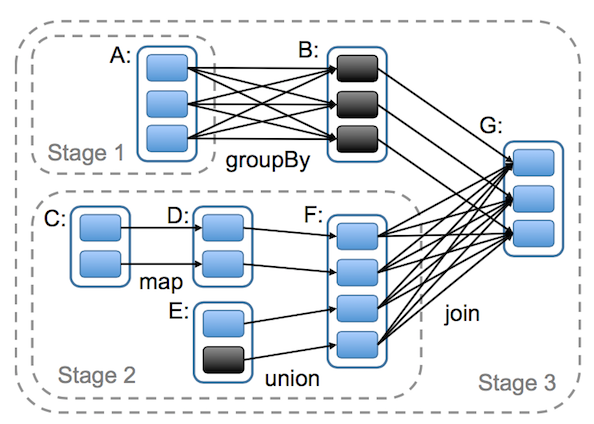
\includegraphics[width=0.9\textwidth]{figures/spark-stage-dag.png}
\caption{Spark:Stage划分算法}
 \label{fig:spark-stage-dag}
\end{figure}

\begin{itemize}
 \item \ascii{Stage 3}的划分
   \begin{enum}
     \eitem{\ascii{G}与\ascii{B}之间是窄依赖,规约为同一\ascii{Stage(3)};}
     \eitem{\ascii{B}与\ascii{A}之间是宽依赖,\ascii{A}为新的起始\ascii{RDD},递归调用此过程;}
     \eitem{\ascii{G}与\ascii{F}之间是宽依赖,\ascii{F}为新的起始\ascii{RDD},递归调用此过程。} 
   \end{enum}

 \item \ascii{Stage 1}的划分
   \begin{enum}
     \eitem{\ascii{A}没有父亲}RDD},\ascii{Stage(1)}划分结束。特殊地\ascii{Stage(1)}仅包含\ascii{RDD A}。}
   \end{enum}
 \item \ascii{Stage 2}的划分
   \begin{enum}
     \eitem{因\ascii{RDD}之间的关系都为窄依赖,规约为同一个\ascii{Stage(2)};}
     \eitem{直至\ascii{RDD C, E},因没有父亲\ascii{RDD},\ascii{Stage(2)}划分结束。}
   \end{enum} 
\end{itemize}

最终,形成了\ascii{Stage}的依赖关系,依次提交\ascii{TaskSet}至\ascii{TaskScheduler}进行调度执行。

\end{content}

\section{独乐乐,不如众乐乐}

\begin{content}

与他人分享你的经验,也许可以找到更多的启发;尤其对于熟知该领域的人沟通,如果是\ascii{Owner}就更好了,肯定能得到意外的惊喜和收获。

也可以通过各种渠道,收集他人的经验,并结合自己的思考,推敲出自己的理解,如此才能将知识放入自己的囊中。

阅读代码,不是一个人的世界;应该走出去,多参加一些社区活动,了解生态圈中主流的研究方向,技术动态,产业发展,对于理解业务是极其有帮助的。


\end{content}

